%%% %%%%%%%%%%%%%%%%%%%%%%%%%%%%%%%% %%%
%%% Main Chapter 4 : Implementation  %%%
%%% %%%%%%%%%%%%%%%%%%%%%%%%%%%%%%%% %%%
\chapter{Setup}
\label{chap:setup}

	In diesem Kapitel wird beschrieben, wie ausgewählte historische Betriebssysteme im Rahem dieser Arbeit wieder lauffähig gemacht wurden. Als Hypervisor kam, sofern nicht anderweitig vermerkt, VMWare Fusion Professional Version 6.0.2 auf Mac OS 10.9.2 zum Einsatz. 
	Die VMs werden zusammen mit dieser Arbeit eingereicht.

%%%%%%%%%%%%%%%%%%%%%%%%%%%%%%%%%%%%%%%%%%%%%%%%%%%%%%%%%%%%%%%%%%%%%%%%%%%%%%%%%%%%%%%%%%%%%%%%%%%%%%%%%
\section{PC DOS 1.10}
%%%%%%%%%%%%%%%%%%%%%%%%%%%%%%%%%%%%%%%%%%%%%%%%%%%%%%%%%%%%%%%%%%%%%%%%%%%%%%%%%%%%%%%%%%%%%%%%%%%%%%%%%

	MS DOS 1.0 stellt das erste Betriebssystem von Microsoft für die 8086-CPU dar. Es entstand durch eine Portierung von Tim Patersons QDOS auf den IBM PC und wurde mit diesem unter dem Namen IBM PC DOS vertrieben. \cite{WinHistory}
	Beim hier verwendeten PC DOS 1.10 handelt es sich um eine fehlerbereinigte, im Juli '82 veröffentlichte Version, die technisch MS DOS 1.25 entspricht. 
	Dieses Betriebssystem stelltgrößtenteils einen Nachbau von CP/M dar und war, außer durch das Vorhandensein des Dateisystems \gls{FAT}, wenig innovativ.
	Da es jedoch die Grundlage für den Erfolg von Microsoft und somit für alle späteren Betriebssysteme bildet, wird es in dieser Arbeit behandelt.

	DOS unterstützt in der Version 1 noch keine Festplatten und kann lediglich 5,25" Disketten bis 160 KB adressieren. \cite{WinHistory}
	Unter anderem aufgrund dieser Einschränkungen kann dieses Betriebssystem nicht mit zeitgemäßen Hypervisoren ausgeführt werden, statt dessen muss ein vollwertiger CPU- bzw. PC-Emulator wie Bochs oder QEMU verwendet werden. 

	\begin{figure}[h]
		\begin{center}
			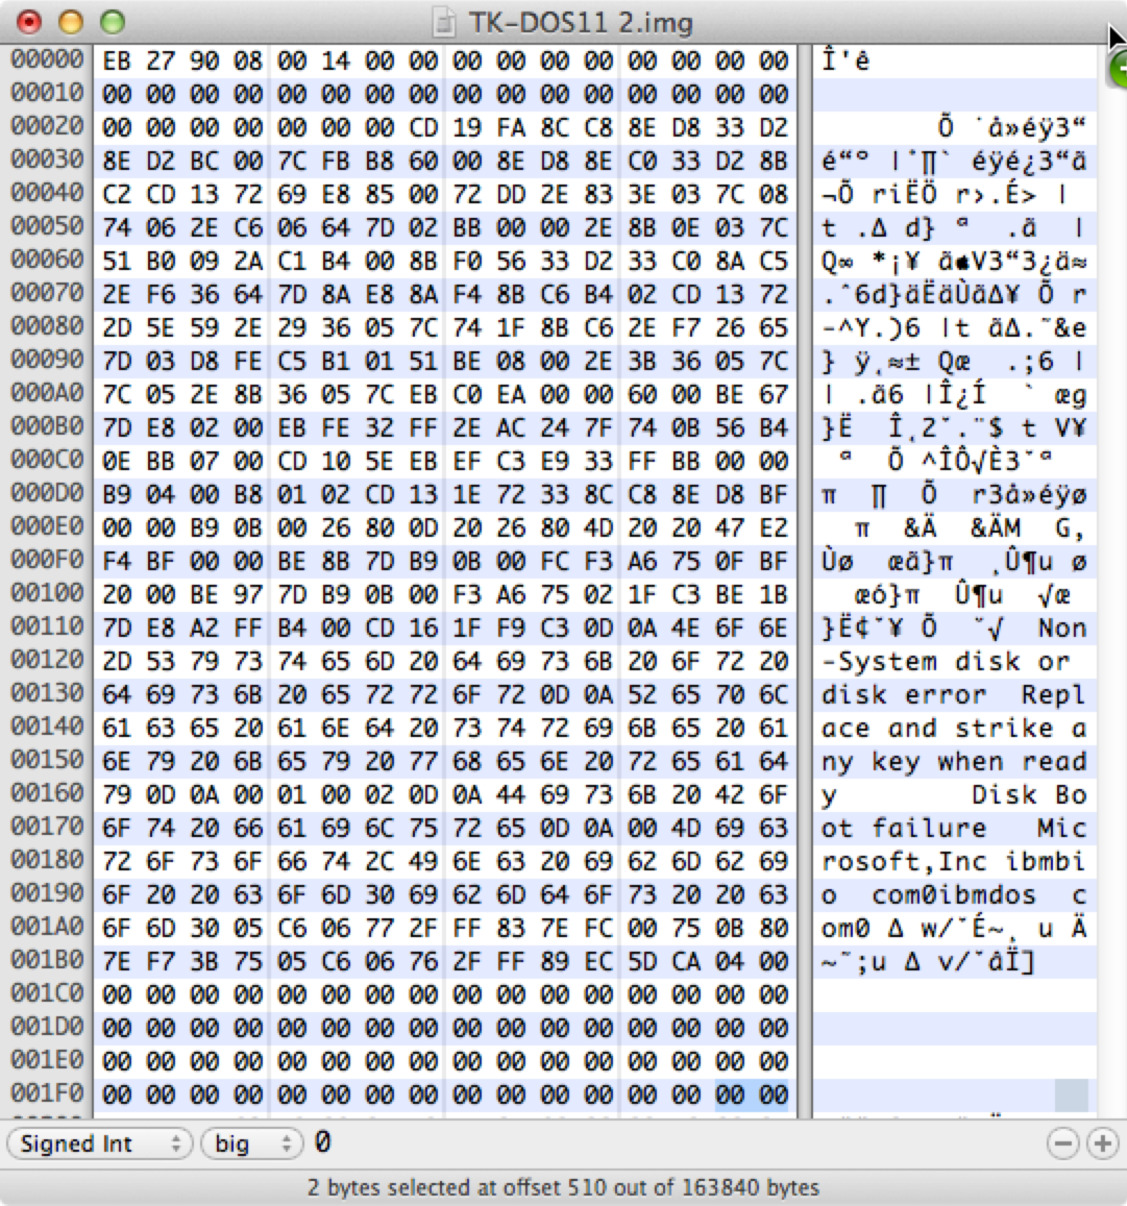
\includegraphics[width=0.6\textwidth]{img/DOS110hex}
			\caption{Ansicht des PC DOS 1.10 Bootsektors im Hex-Editor}
			\label{fig:screenshot-hexeditor110}
		\end{center}
	\end{figure}

	Im "`Endangered Software Archive"', welches unter der URL \url{http://www.mirrors.org/archived_software/www.techknight.com/esa/default.htm} verfügbar ist, befindet sich eine mit dem "`Disk Image Archiver"' erstellte Kopie der originalen PC DOS 1.10 Startdiskette. 
	Mit einem Hex-Editor lässt sich aus dem proprietären .dim-Format eine Datei mit dem Inhalt der Diskette erstellen und das Betriebssystem in Bochs booten.
	Dieser Prozess ist in \cite{PCMinistry} beschrieben:

	Der Bootsektor der Diskette entspricht noch nicht den gängingen Industriestandards.
	So fehlt der BIOS Parameter Block, der bei allen FAT (ab DOS 2.0) und NTFS Dateisystemen den Aufbau des Datenträgersbeschreibt und Informationen über das Dateisystem enthält. Im vorliegenden Image ist dieser Bereich (ab Offsett 07h) freigelassen.
	Modernere Betriebssysteme können die Diskette daher nicht lesen und geben aus, der Datenträger sei nicht korrekt formattiert. 
	Zudem wird die "`Boot Sektor Signatur"' am Ende des ersten Sektors (55h bei Offsett 1FEh und AAh bei Offsett 1FFh), welche ein Medium als bootbar markiert, vom BIOS bei Start noch nicht überprüft. \cite{IBMTechRef} Daher fehlt auch diese auf der Diskette und in dem Image sind am Ende des Bootsektors lediglich Nullen zu finden.
	Daher verweigert der Emulator den Bootvorgang.
	Ändert man mit einem Hex-Editor die Datei und schreibt 55AA an das Ende des Bootsektors, übergibt das BIOS die Kontrolle mittels JMP-Befehl an den in dem Image liegenden Code. Leider stürzt das System dann beim Bootvorgang ab.

	Glücklicherweise bietet Bochs bietet jedoch die Möglichkeit, die Überprüfung der Signatur zu deaktivieren und jeglichen Programmcode sofort zu booten, indem man \lstinline{floppy_bootsig_check: disabled=1} in das config file schreibt.
	Ein funktionierendes config File wird unter dem Namen $bochs.txt$ mit dieser Arbeit ausgeliefert.
	Hiermit lässt sich ein unverändertes Image von PC DOS 1.10 ausführen.
	Hierzu muss bochs im entsprechenden Verzeichnis gestartet werden, die Option \lstinline{2. Read options from...} gewählt werden, mittels \lstinline{6. Begin simulation} der Emulator geladen werden und mit dem Befehl $continue$ die CPU gestartet werden.

	\begin{figure}[p]
		\begin{center}
			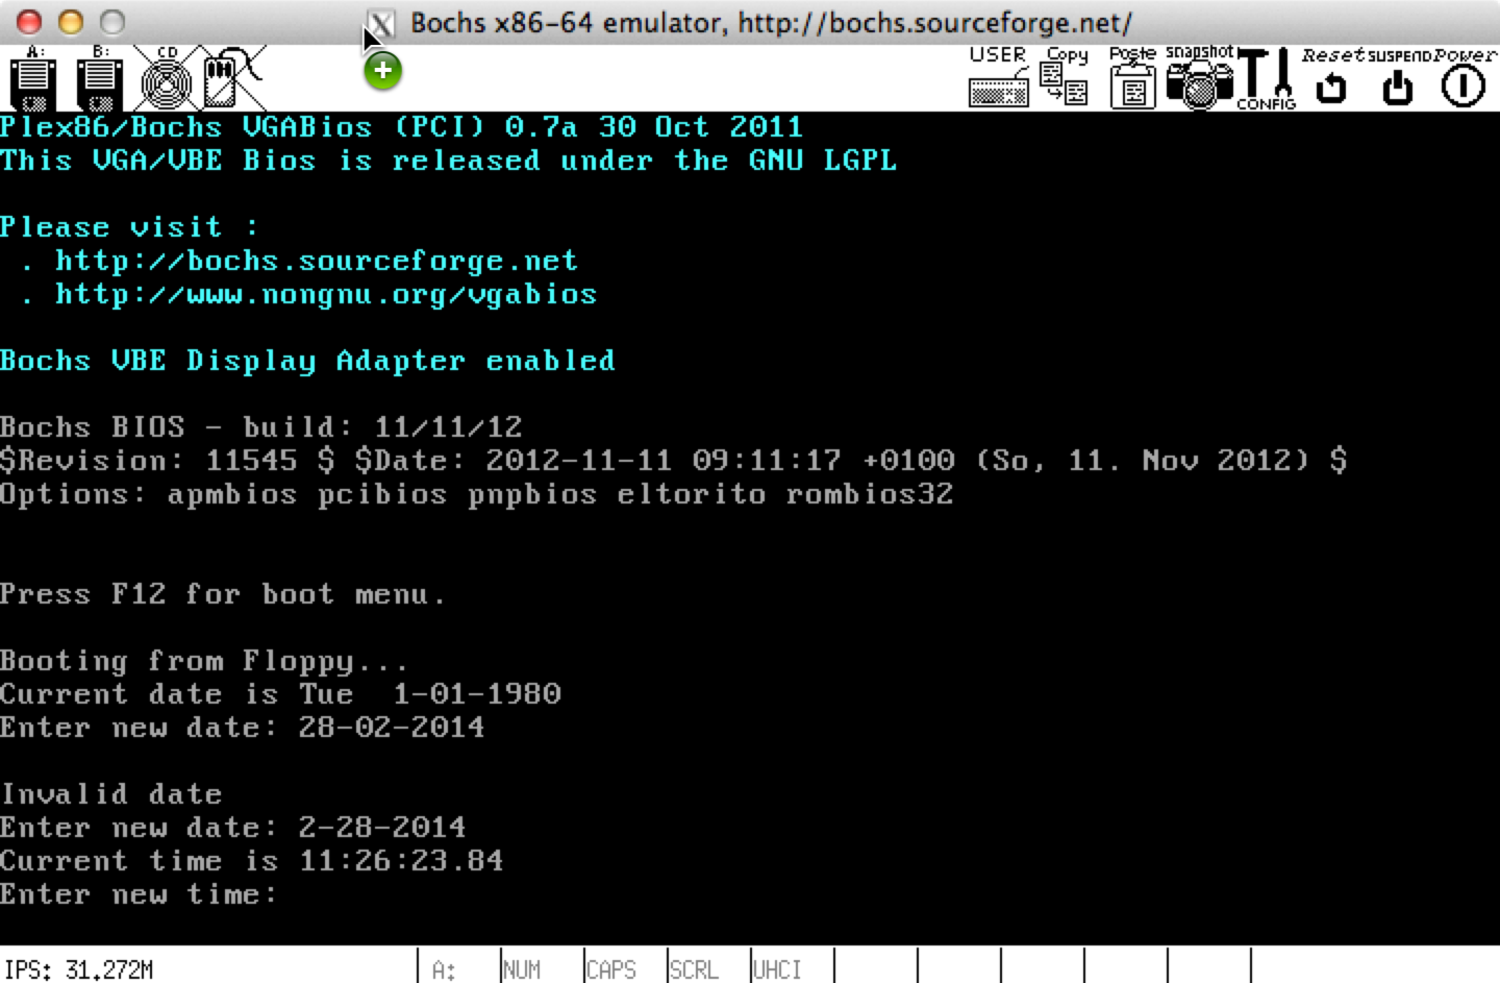
\includegraphics[width=\textwidth]{img/DOS110_1}
			\caption{Bootscreen von DOS 1.10}
			\label{fig:screenshot-dos110boot}
		\end{center}
	\end{figure}

	\begin{figure}[p]
		\begin{center}
			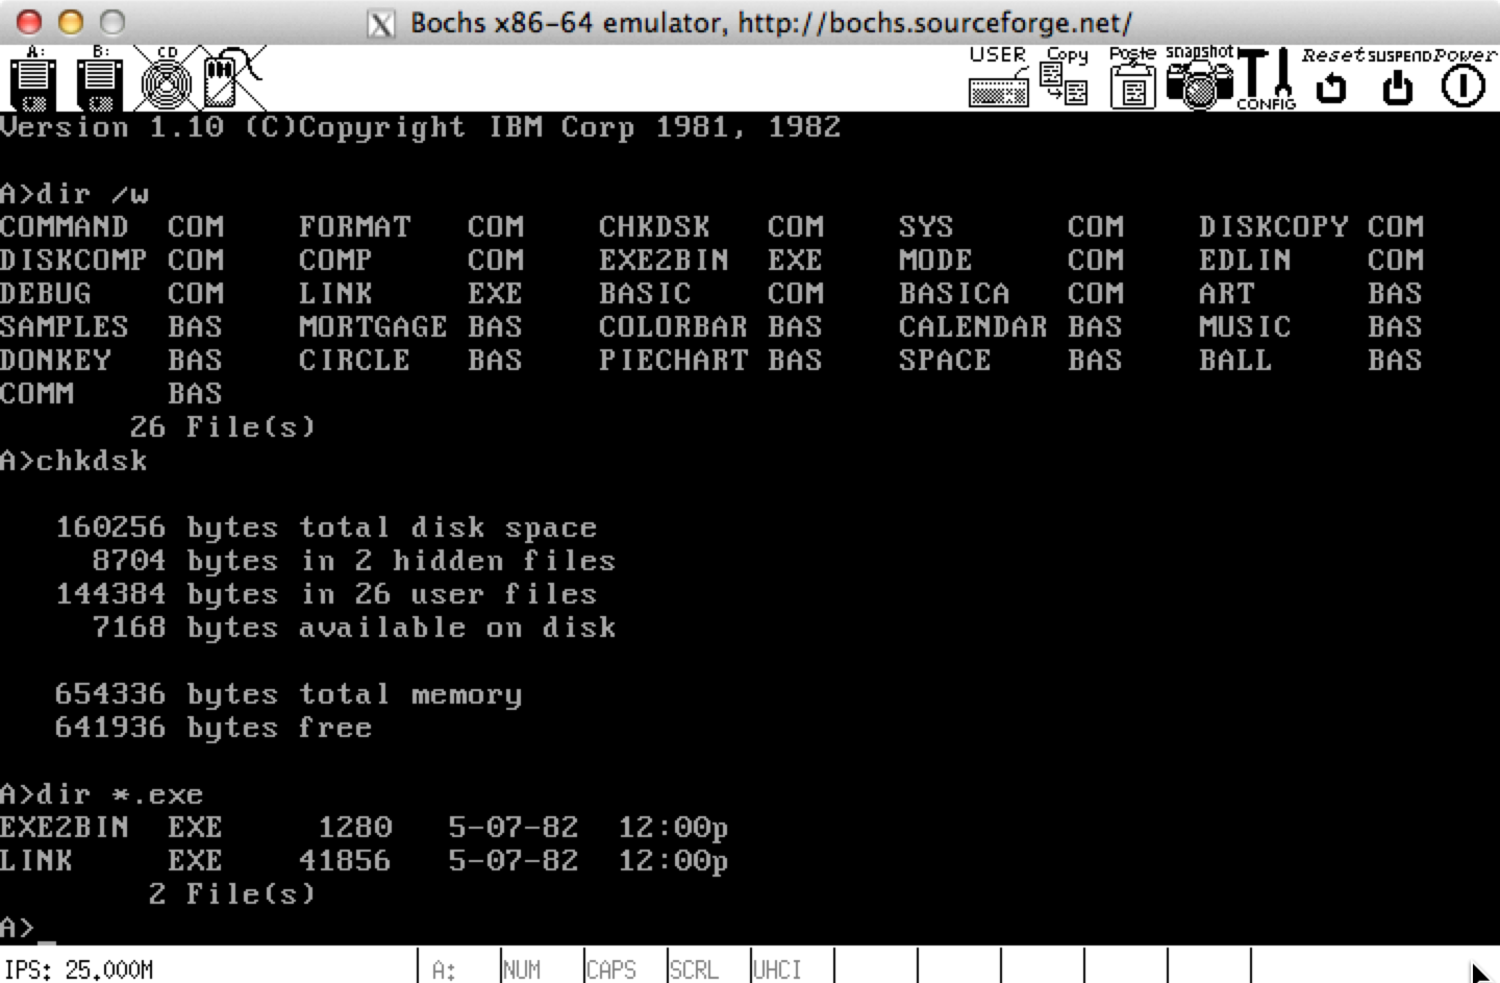
\includegraphics[width=\textwidth]{img/DOS110_2}
			\caption{Kommandos in PC DOS 1.10}
			\label{fig:screenshot-dos110commands}
		\end{center}
	\end{figure}

	Leider sind auch hier bei weitem nicht alle Funktionen des Betriebssystems benutzbar, da MS DOS sämtliche I/O-Operationen über die BIOS-Routinen durchführt.
	Das im originalen IBM PC verwendete BIOS unterscheidet sich jedoch signifikant von der "`BIOS Boot Specification"' vom 11. Januar 1996 und ist daher mit dem verwendeten Plex86/Bochs VGABios nicht kompatibel.


%%%%%%%%%%%%%%%%%%%%%%%%%%%%%%%%%%%%%%%%%%%%%%%%%%%%%%%%%%%%%%%%%%%%%%%%%%%%%%%%%%%%%%%%%%%%%%%%%%%%%%%%%
\section{DOS 5.0 \& Windows 2.11}
%%%%%%%%%%%%%%%%%%%%%%%%%%%%%%%%%%%%%%%%%%%%%%%%%%%%%%%%%%%%%%%%%%%%%%%%%%%%%%%%%%%%%%%%%%%%%%%%%%%%%%%%%


%%%%%%%%%%%%%%%%%%%%%%%%%%%%%%%%%%%%%%%%%%%%%%%%%%%%%%%%%%%%%%%%%%%%%%%%%%%%%%%%%%%%%%%%%%%%%%%%%%%%%%%%%
\section{DOS 6.0 \& Windows 3.11}
%%%%%%%%%%%%%%%%%%%%%%%%%%%%%%%%%%%%%%%%%%%%%%%%%%%%%%%%%%%%%%%%%%%%%%%%%%%%%%%%%%%%%%%%%%%%%%%%%%%%%%%%%


%%%%%%%%%%%%%%%%%%%%%%%%%%%%%%%%%%%%%%%%%%%%%%%%%%%%%%%%%%%%%%%%%%%%%%%%%%%%%%%%%%%%%%%%%%%%%%%%%%%%%%%%%
\section{Windows NT 3.51}
%%%%%%%%%%%%%%%%%%%%%%%%%%%%%%%%%%%%%%%%%%%%%%%%%%%%%%%%%%%%%%%%%%%%%%%%%%%%%%%%%%%%%%%%%%%%%%%%%%%%%%%%%


%%%%%%%%%%%%%%%%%%%%%%%%%%%%%%%%%%%%%%%%%%%%%%%%%%%%%%%%%%%%%%%%%%%%%%%%%%%%%%%%%%%%%%%%%%%%%%%%%%%%%%%%%
\section{Windows NT 4.0 SP 6}
%%%%%%%%%%%%%%%%%%%%%%%%%%%%%%%%%%%%%%%%%%%%%%%%%%%%%%%%%%%%%%%%%%%%%%%%%%%%%%%%%%%%%%%%%%%%%%%%%%%%%%%%%


%%%%%%%%%%%%%%%%%%%%%%%%%%%%%%%%%%%%%%%%%%%%%%%%%%%%%%%%%%%%%%%%%%%%%%%%%%%%%%%%%%%%%%%%%%%%%%%%%%%%%%%%%
\section{Windows 2000 Professional}
%%%%%%%%%%%%%%%%%%%%%%%%%%%%%%%%%%%%%%%%%%%%%%%%%%%%%%%%%%%%%%%%%%%%%%%%%%%%%%%%%%%%%%%%%%%%%%%%%%%%%%%%%
